\documentclass[runningheads,a4paper]{llncs}

\usepackage{amssymb}
\setcounter{tocdepth}{3}
\usepackage{graphicx}


\usepackage{url}
\usepackage{algpseudocode}
\usepackage{algorithm}
\usepackage{algorithmicx}



\urldef{\mailsa}\path|gorohov.art@gmail.com|    
\newcommand{\keywords}[1]{\par\addvspace\baselineskip
\noindent\keywordname\enspace\ignorespaces#1}

%To economize paper
%\textwidth=190mm
%\textheight=250mm
%\topmargin=-20mm
%\oddsidemargin=-15mm
%\evensidemargin=-15mm


\begin{document}

\algnewcommand\algorithmicswitch{\textbf{switch}}
\algnewcommand\algorithmiccase{\textbf{case}}
\algnewcommand\algorithmicassert{\texttt{assert}}
\algnewcommand\Assert[1]{\State \algorithmicassert(#1)}
% New "environments"
\algdef{SE}[SWITCH]{Switch}{EndSwitch}[1]{\algorithmicswitch\ #1\ \algorithmicdo}{\algorithmicend\ \algorithmicswitch}
\algdef{SE}[CASE]{Case}{EndCase}[1]{\algorithmiccase\ #1}{\algorithmicend\ \algorithmiccase}

\algtext*{EndSwitch}
\algtext*{EndCase}
\algtext*{EndWhile}% Remove "end while" text
\algtext*{EndIf}% Remove "end if" text
\algtext*{EndFor}% Remove "end for" text
\algtext*{EndFunction}% Remove "end function" text

\newtheorem{mydef}{Definition}

\mainmatter  % start of an individual contribution

% first the title is needed
\title{EBNF in GLL}

% a short form should be given in case it is too long for the running head
\titlerunning{EBNF in GLL}

\author{Artem Gorokhov}
\authorrunning{Artem Gorokhov}
% (feature abused for this document to repeat the title also on left hand pages)

\institute{St. Petersburg State University, Universitetsky prospekt, 28,\\
           198504 Peterhof, St. Petersburg, Russia\\
\mailsa}

\toctitle{EBNF in GLL}
\tocauthor{Artem Gorokhov}
\maketitle

%Authors are invited to submit full papers (not exceeding 12 pages) or short papers (up to 6 pages)

\begin{abstract}
% Предлагается модификация алгоритма GLL, работающая с грамматиками в форме EBNF. 
% Это приносит ошутимый прирост производительности в работе с некоторыми грамматиками языков программирования.

At least 70 and at most 150 words.
word0 word1 word2 word3 word4 word5 word6 word7 word8 word9
word0 word1 word2 word3 word4 word5 word6 word7 word8 word9
word0 word1 word2 word3 word4 word5 word6 word7 word8 word9
word0 word1 word2 word3 word4 word5 word6 word7 word8 word9
word0 word1 word2 word3 word4 word5 word6 word7 word8 word9
word0 word1 word2 word3 word4 word5 word6 word7 word8 word9
word0 word1 word2 word3 word4 word5 word6 word7 word8 word9
word0 word1 word2 word3 word4 word5 word6 word7 word8 word9
word0 word1 word2 word3 word4 word5 word6 word7 word8 word9
word0 word1 word2 word3 word4 word5 word6 word7 word8 word9
word0 word1 word2 word3 word4 word5 word6 word7 word8 word9
word0 word1 word2 word3 word4 word5 word6 word7 word8 word9
word0 word1 word2 word3 word4 word5 word6 word7 word8 word9

\keywords{Parsing, GLL, EBNF}
\end{abstract}


\section{Introduction}%--------------------------------------------------------------------------------------------------------------------------------------------

Static program analysis usually performed over structural representation of code and parsing is a classical way to get such representation.
Parser generators often used for parser creation automation: these tools allow to create parser from grammar of language which should be specified in appropreate format.
It allows to decrease efforts required for syntax analyzer creation and maintenance.

Extended BNF (EBNF) is a useful format of grammar specification. 
Expressive and compact description of language sintax. 
This formalism often used in documentation --- one of main source of information for parsers developers.

There are a wide range of parsing techniques and algorithms: CYK, LR(k), LALR(k), LL, etc. 
One of he most popular area is generalized parsing: technique which allows to handle ambiguous grammars. 
It is possible to simplify language description required for parser generation in case if parser generator is based on generalized algorithm.
LL family is more intutively than LR, can provide better diagnostics, but LL(1) is not enough to process some languages: there are LR, but not LL languages.
Moreover, left and hidden left recursion in grammars is a problem. 
In order to solve these problems generalized LL (GLL) was proposed~\cite{!!!}. 
This algorithm handles arbitrary context free grammar, even anaumbiguos and (hidden)left-recursve.
Worst-case time and space complexity of GLL is cubic in terms of input size. 
For LL grammars it demonstartes linear time and space complexity.

But BNF required for classical parsing algorithms.
It is possible to convert from EBNF to BNF but ....

ELL, ELR~\cite{AttributedELL,ELRR,ECFGparsing,ELLParser,ELL,ECFG,ELALR,ELRParsing} and other can process EBNF but what about ambiguities in grammars. It is a problem.

Factorization for GLL, but it is not full support of EBNF.

In this work we present modified generalized LL parsing algorithm which handles grammars in EBNF without transformations.
Changes are very native for GLL nature.
Proposed modifications allow to get sufficient parsing performance improvement.

This article is structurerd as follows.
We start from .... Extended BNF
generalized LL algorithm description.
Blah-blah


%Синтаксический анализ программ это широко известная область, ...
%Проблема в том, что грамматики, используемые в реальной жизни пишутся в форме EBNF. А GLL принимает только BNF.
%Можно проводить преобразование грамматики из EBNF к BNF, но так она разрастается, что, в некоторых случаях, замедляет процедуру разбора.
%Предлагается модификация алгоритма GLL, работающая с грамматиками в форме EBNF.



\section{EBNF processing}

EBNF definition

Extended Backus-Naur Form~\cite{iso} is a syntax of expressing context-free grammars. Unlike the Backus-Naur Form it 
uses such new constructions:
\begin{itemize}
    \item alternation $\mid$
    \item option [ ... ]
    \item repetition \{ ... \}
    \item grouping ( ... )
\end{itemize}

It allows to define grammars in more compact way.

Regular expression syntax? Look at ``Towards a Taxonomy for ECFG and RRPG Parsing''

In this article we will use the next notation: ....

ELL, ELR etc


\section{Generalized LL Parsing}%--------------------------------------------------------------------------------------------------------------------------------------------

Basic GLL algorithm~\cite{scott2010gll} allows to perform syntax analysis of linear input by any context-free 
grammar. As a result we get Shared Packed Parse Forest(SPPF)~\cite{SPPF} that represents all possible derivations of input string.

Work of the GLL algorithm based on descriptors. Descriptor is a four-element tuple that can uniquely define state 
of parsing process. It consists of:
\begin{itemize}
    \item \textbf{Slot} --- position in grammar
    \item \textbf{Position in input} graph
    \item Already built \textbf{tree root}
    \item Current \textbf{GSS node}
\end{itemize}

and so on about GLL

\subsection{Factorization}%--------------------------------------------------------------------------------------------------------------------------------------------

Elizabeth Scott and Adrian Johnstone offered support of factorised grammars in GLL~\cite{scott2016structuring}. 
But our approach yields more increase in performance on some grammars


\section{Extended BNF GLL Parsing}%--------------------------------------------------------------------------------------------------------------------------------------------

In this section we will show an application of Extended Backus-Naur Form(EBNF) grammars in automatons and corresponding GLL-style parsers.

GLL allows analysis only by grammars in Backus-Naur Form. When use of EBNF is more common.

Main algorithm creates and queues new descriptors depending on current parse state that we get from unqueued descriptor. 
In case descriptor was already created it does not add it to queue. For this purpose we have a set of
\textbf{all} created descriptors. Thus reducing set of possible descriptors decreases the parse time
and required memory.

Let us spot on \textbf{slots}. Grammar written in EBNF is usually more compact then it's representation in BNF. That means EBNF contains 
less slots and parser creates less descriptors. Thus support of EBNF in GLL can increase parsing performance. 


\subsection{Grammar Transformation}%--------------------------------------------------------------------------------------------------------------------------------------------

There are some basic methods converting regular expressions to nondeterministic finite state automatons. 
At the same time context-free grammar productions are regular expressions, that can contain as terminals 
as nonterminals. Thus for each grammar rule we can build a finite state automaton, with edges tagged with 
terminals, nonterminals or $\varepsilon$-symbols. We used Thompson's method~\cite{Thompson:1968:PTR:363347.363387}. 
In built automatons nonterminals should be replaced with links to initial states of automaton that stands 
for this nonterminal. An example of constructed automaton for grammar $\Gamma_{0}$\ref{fig:grammarG0} is given on fig.

Produced $\varepsilon$-NFAs can be converted to DFAs. An algorithm is described in~\cite{aho1974design}.

Minimization of the quantity of the DFA states decreases number of GLL descriptors. John Hopcroft's 
algorithm~\cite{hopcroft1971n} can be used for it. But we can apply it to all automatons at one time. 
An algorithm is based on dividing all states on equivalent classes. Initial state of algorithm consist 
of 2 classes: first contains final states and second contains all other. For our problem we can set an 
initial state as follow: first class contains all final states of \textbf{all} automatons and second class 
contains all the other. As an algorithm result we get classes which represent states of minimised DFA and 
transitions between them.
Initial state is class that contains initial state of automaton that represents productions of start nonterminal.
% Надо сказать про то что на самом деле структура грамматики не меняется. Меняется лишь её представление.

Some states have labels: names of nonterminals which productions start in that states.


\subsection{Input processing}%--------------------------------------------------------------------------------------------------------------------------------------------

Slots becomes DFA states. And just as we can move through grammar slots we can move through states 
in DFA. But in DFA we have multiple ways to go because many nonterminals can start with current input symbol. 
%So we need to prevent creation of descriptors for each nonterminal on out edges. We can generate tables that 
%tells us what nonterminals can infer strings that starts with current terminal. And add descriptors only for 
%this edges. Moreover we need to create descriptor for edge that marked with current terminal if such exists.


\begin{algorithmic}
\Function{add}{$S,u,i,w$}
    \If{$(S,u,i,w) \notin U$}  
        \State $U.add(S,u,i,w)$
        \State $R.add(S,u,i,w)$
    \EndIf
\EndFunction
\end{algorithmic}
\begin{algorithmic}    
\Function{create}{$edge, u, i, w$}
    \State $(\underline{\hspace{0.25cm}}, Nonterm(A, S_{call}), S_{next})) \gets edge$
    \If{($\exists$ GSS node labeled $(A, i)$)}  
    
        \State $v \gets$ GSS node labeled $(A, i)$
        \If{(there is no GSS edge from $v$ to $u$ labeled ($S_{next},w$))}
            \State add a GSS edge from $v$ to $u$ labeled ($S_{next},w$)
            \For{($(v, z) \in \mathcal{P} $)}
                \State $(y,N) \gets$ \textbf{getNodes}($S_{next}, u.nonterm, w, z$)
                \If{$N \neq \$$}
                    \State $(\_, \_, h) \gets N$
                    \State \textbf{pop}$(u,h,N)$ 
                \EndIf
                
                \State $(\_, \_, h) \gets y$
                \State \textbf{add}($S_{next} , u, h, y$)
                
            \EndFor
        \EndIf
    
    \Else
        \State $v \gets$ \textbf{new} GSS node labeled $(A, i)$
        \State create a GSS edge from $v$ to $u$ labeled ($S_{next}, w$)
        \State \textbf{add}($S_{call}, v, i, \$ $)
    \EndIf
    \Return{$v$}
\EndFunction
\end{algorithmic}  

\begin{algorithmic}   
\Function{pop}{$u,i,z$}
    \If{($(u,z) \notin \mathcal{P}$)}  
        \State $\mathcal{P}.add(u,z)$
        \ForAll{GSS edges $(u,S,w,v)$}
            \State $(y,N) \gets$ \textbf{getNodes}($S, v.nonterm, w, z$)
            \State \textbf{add}($S,v,i,y$)
            \If{$N \neq \$$}
                \ \textbf{pop}$(v,i,N)$ 
            \EndIf
        \EndFor
    \EndIf
\EndFunction
\end{algorithmic}


\subsection{SPPF construction}

First, we should define derivation trees for DFA's: it is an ordered tree whose root is lable of the start state,
leaf nodes are labeled with a terminals from DFA's edges or $\varepsilon$ and interior nodes are labeled with 
nonterminals from DFA's edges($ A $) and have a sequence of children that corresponds to edge labels of path in 
DFA that starts from the state labeled $ A $. More formal. 

\begin{mydef}

Derivation tree of sentence $\alpha$ in the grammar $G=(\Sigma, N, S, P)$:

\begin{itemize}
\item Ordered rooted tree. Root labeled with $S$
\item Leafs are terminals $\in \Sigma$
\item Nodes is nonterminals
\item Node with label $N_i$ has childs $l_0, \dots\, l_n$ if and only if for $\omega = l_0 \cdot l_1 \dots\ l_n\in (\Sigma \cup N)^*$ exists $p \rightarrow M \in P$ such that $\omega \in L(M)$
\end{itemize}

\end{mydef}

DFA is ambiguous if there exist string that have more than one derivation trees. Thus, we can define SPPF for DFA. 
It is similar to SPPF for grammars described in~\cite{scott2013gll}. SPPF contains symbol nodes(like derivation trees), packed nodes
and intermediate nodes. 

Packed nodes are of the form $(S, k)$, where $S$ is a state of DFA. 
Symbol nodes have labels $(X, i, j)$ where $X$ is an edge symbol or a nonterminal. 
Intermediate nodes have labels $ (S, i, j) $, where $S$ is a state of DFA

A packed node has one or two children right child can be symbol node, left child can be symbol or intermediate node.   
Nonterminal symbol nodes have packed children nodes of the form $(S, k)$ where $S$ is pop state. 
Terminal symbol nodes are leafs.

 Use of intermediate and packed nodes leads to binarization of SPPF and thus the space complexity is $O(n^{3})$.
%But in grammars slot defines position,
%previous and next symbol, when DFA state tells the position only. Thus we can can construct SPPF using 
%In general, we can't uniquely correspond an original grammar slot to automaton state.
%We can consider example. For the grammar \ref{fig:grammarG0}, automaton will be represented as showed on fig.\ref{fig:automatonForG0}.
%SPPF for input "aa" is on fig.\ref{fig:SPPF}.

\begin{figure}
    \centering
    \parbox{2.9cm}{
        \begin{center}
            $S ::= (aa)|(ab)$
        \end{center}
        \caption{Grammar $\Gamma_{0}$}
        \label{fig:grammarG0}}
    \qquad
    \begin{minipage}{4cm}
        \includegraphics[width=4cm]{pictures/automatonForG0.pdf}
        \caption{Automaton for $\Gamma_{0}$}
        \label{fig:automatonForG0}
    \end{minipage}
\end{figure}

\begin{figure}
    \centering
    \includegraphics[width=4cm]{pictures/SPPFforG0.pdf}
    \caption{SPPF for input "aa"}
    \label{fig:SPPF}
\end{figure}


State 1 can be matched with two grammar slots: $S ::= (a \cdot a)|(b$ $a)$ and $S ::= (a$ $a)|(b \cdot a)$. 
But SPPF represents WHAT???




\textbf{function} getNodeT$(x,i)$ does not change

In states of parsing we can have a nondeterministic choice because the states of DFA can be ``pop'' states.
In this case we need to create nonterminal node and raise \textbf{pop} function. But if there exist out edges from this state we also need to create intermediate node.
For this purpose we defined function \textbf{getNodes} which can construct two nodes: intermediate and nonterminal (at least one of them, at most both of them).
So if current state is ``pop'' state it constructs nonterminal node

\begin{algorithmic}
\Function{getNodes}{$S, A, w, z$}
    \If{($S$ is final state)}
        \State $x \gets \textbf{getNodeP}(S, A, w, z)$
    \Else
        \State $x \gets \$ $
    \EndIf
    \Statex
    %\If{$S.outedges = \varnothing$}
    %    \State $y \gets \$$
    %\Else
        \If{$(w = \$) \&$ not ($z$ is nonterminal node and it's extents are equal)}
            \State $y \gets z$
        \Else
            \State $y \gets \textbf{getNodeP}(S, S, w, z)$
        \EndIf
    %\EndIf
    
    \State \Return{$(y,x)$}
\EndFunction   
\end{algorithmic}
\begin{algorithmic}
\Function{getNodeP}{$S, L, w, z$}
    \State $(\underline{\hspace{0.25cm}}, k, i) \gets z$
    
    \If{($w \neq \$$)}
        \State $(\underline{\hspace{0.25cm}}, j, k) \gets w$
    
        \State $y \gets$ find or create SPPF node labelled $(L, j, i)$  
    
        \If{($\nexists$ child of $y$ labelled $(S, k)$)}
            \State $y\prime \gets \textbf{new}$ $packedNode(S, k)$
            \State $y\prime.addLeftChild(w)$
            \State $y\prime.addRightChild(z)$
            \State $y.addChild(y\prime)$
        \EndIf
    
    \Else
        \State $y \gets$ find or create SPPF node labelled $(L, k, i)$ 
        \If{($\nexists$ child of $y$ labelled $(S, k)$)}
            \State $y\prime \gets \textbf{new}$ $packedNode(S, k)$
            \State $y\prime.addRightChild(z)$
            \State $y.addChild(y\prime)$
        \EndIf
    \EndIf
    \State \Return{$y$}
\EndFunction
\end{algorithmic}
\begin{algorithmic}
\Function{parse}{}
    \State $R.add(StartState, new GSSnode(StartNonterminal,0), 0, \$)$
    \While{$R \neq \varnothing $}
    \State{$(C_{S},C_{U},C_{i},C_{N}) \gets R.Get()$}
    \State{$C_{R} \gets \$$}
    
    \If{$(C_{N} = \$) \& (C_{S}$ is pop state)}
    \State $eps \gets \textbf{getNodeT}(\varepsilon, C_{i})$  
    \State $(\underline{\hspace{0.25cm}}, N) \gets \textbf{getNodes}(C_{S},C_{U}.nonterm, \$, eps)$
    \State \textbf{pop}$(C_{U},C_{i},N)$ 
    \EndIf
    
    \For{\textbf{each} $edge (C_{S},symbol,S_{next})$}
        \Switch{$symbol$}  
        \Case{$Terminal(x)$ where ($x = input[i]$)}
            \State $C_{R} \gets \textbf{getNodeT}(x, C_{i})$
            
            \State{$C_{i} \gets C_{i} + 1$}
                        
            \State $(C_{N}, N) \gets \textbf{getNodes}(S_{next},C_{U}.nonterm, C_{N}, C_{R})$
            \If{$N \neq \$$}
                \State \textbf{pop}$(C_{U},C_{i},N)$ 
            \EndIf
            
            \If{$C_{N} \neq \$$}
                \State $R.add(S_{next}, C_{N}, C_{i}, C_{N})$
            \EndIf
            
        \EndCase
    
        \Case{$Nonterminal(A, S_{call})$}
    %\State{$slots \gets pTable[A][input[i]]$}
    %\If{$slots \neq \varnothing$}
            \State \textbf{create}($edge, C_{U}, C_{i}, C_{N}$)
    %\EndIf
    %\ForAll{$L \in slots$}
    %    \State{\Call{add}{L,u,i,\$}} 
    %\EndFor
        \EndCase
        \EndSwitch
        
    \EndFor
    \EndWhile
\EndFunction
\end{algorithmic}


\section{Evaluation}

Left factorization vs EBNF

Small demo example (message to Scott)

\begin{figure}[h]
$$
\begin{array}{crcl}
& \mbox{\texttt{ S }} &::=& \mbox{\texttt{ A A A A A A | A a A A A A }} \\
& \mbox{\texttt{ A }} & ::=& \mbox{\texttt{ S A | a A | a}}\\
\end{array}
$$
\caption{Grammar $G_0$.}
\label{testGrammar}
\end{figure}

We have compared our parsers built on factorized grammar and on minimized FSA. Grammar $G_0$(fig.~\ref{testGrammar}) was used for the tests. FSA built for this grammar presented on fig.~\ref{dfa}.

Note: SPPF construction was disabled while testing.

\begin{table}[h]
\begin{center}
  \begin{tabular}{ | l | l | l | l | l | l | l | l | l | }
\hline
    Length & \multicolumn{2}{ c| }{Time, seconds} & \multicolumn{2}{ c| }{Descriptors} & \multicolumn{2}{ c| }{GSS Nodes} & \multicolumn{2}{ c| }{GSS Edges} \\ \hline
     & factorized & minimized & factorized & minimized & factorized & minimized & factorized & minimized \\ \hline
    100 & 0.206 & 0.127 & 52790 & 38530 & 200 & 200 & 42794 & 28534 \\ \hline
    200 & 1.909 & 1.54 & 215540 & 157030 & 400 & 400 & 175544 & 117034 \\ \hline
    300 & 8.844 & 7.125 & 488290 & 355530 & 600 & 600 & 398294 & 265534 \\ \hline
    400 & 25.876 & 21.707 & 871040 & 634030 & 800 & 800 & 711044 & 474034 \\ \hline
    500 & 60.617 & 51.245 & 1363790 & 992530 & 1000 & 1000 & 1113794 & 742534 \\ \hline
    1000 & 842.779 & 768.853 & 5477540 & 3985030 & 2000 & 2000 & 4477544 & 2985034 \\ \hline
     & \multicolumn{2}{ c| }{Average gain: 19$\%$} & \multicolumn{2}{ c| }{Average gain: 27$\%$} & \multicolumn{2}{ c| }{Average gain: 0$\%$} & \multicolumn{2}{ c| }{Average gain: 33$\%$} \\ \hline
\end{tabular}
\end{center}
\caption{Experiments results.}
\label{expTable}
\end{table}

Table~\ref{expTable} shows that in general minimized version works $19\%$ faster, uses $27\%$ less descriptors and $33\%$ less GSS edges.
Also we use this FSA approach in metagenomic assemblies parsing and it gives us visible performance increase. Furthermore we can use EBNF constructions without any conversion.

What do you think about this idea and results? 



\section{Conclusion and Future Work}

Described allgorithm implemented in F\# as part of the YaccConstructor project.
Source code available here:\url{!!!}.

Graph parsing, bioinformatics...

Moreover there is a modification that allows to use it with regular approximations It was introduced by 
Anastasia Ragozina in her master's thesis.


Attributed grammar and semantic calculation.


\bibliographystyle{abbrv}
\bibliography{bibliography}
\appendix

\section{\appendixname: Example of parsing and SPPF construction}\label{example}

We demonstrate the application of our algorithm by the following example. The reference grammar is shown below:

$$
\begin{array}{crcl}
(0)& start\_rule &::=& s \\
(1)& s & ::= & \mbox{\texttt{LBR }} s \mbox{\texttt{ RBR }} s\\
(2)& s & ::= &\epsilon
\end{array}
$$

The automaton for regular approximation after tokenization is shown on the Fig.~\ref{faApprox}; the 
SPPF, provided by our algorithm, is shown on the Fig.~\ref{resultSPPF}.

 \begin{figure}[!ht]
    \subfloat[Regular approximation for string-embedded code after tokenization\label{faApprox}]{%
      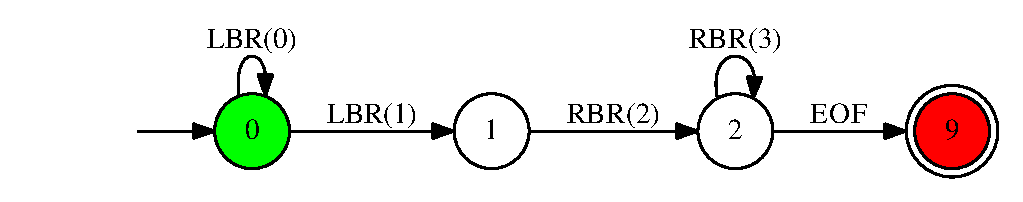
\includegraphics[scale=0.3]{dot/in3.eps}
   }  
   \hfill
    \subfloat[SPPF\label{resultSPPF}]{%
      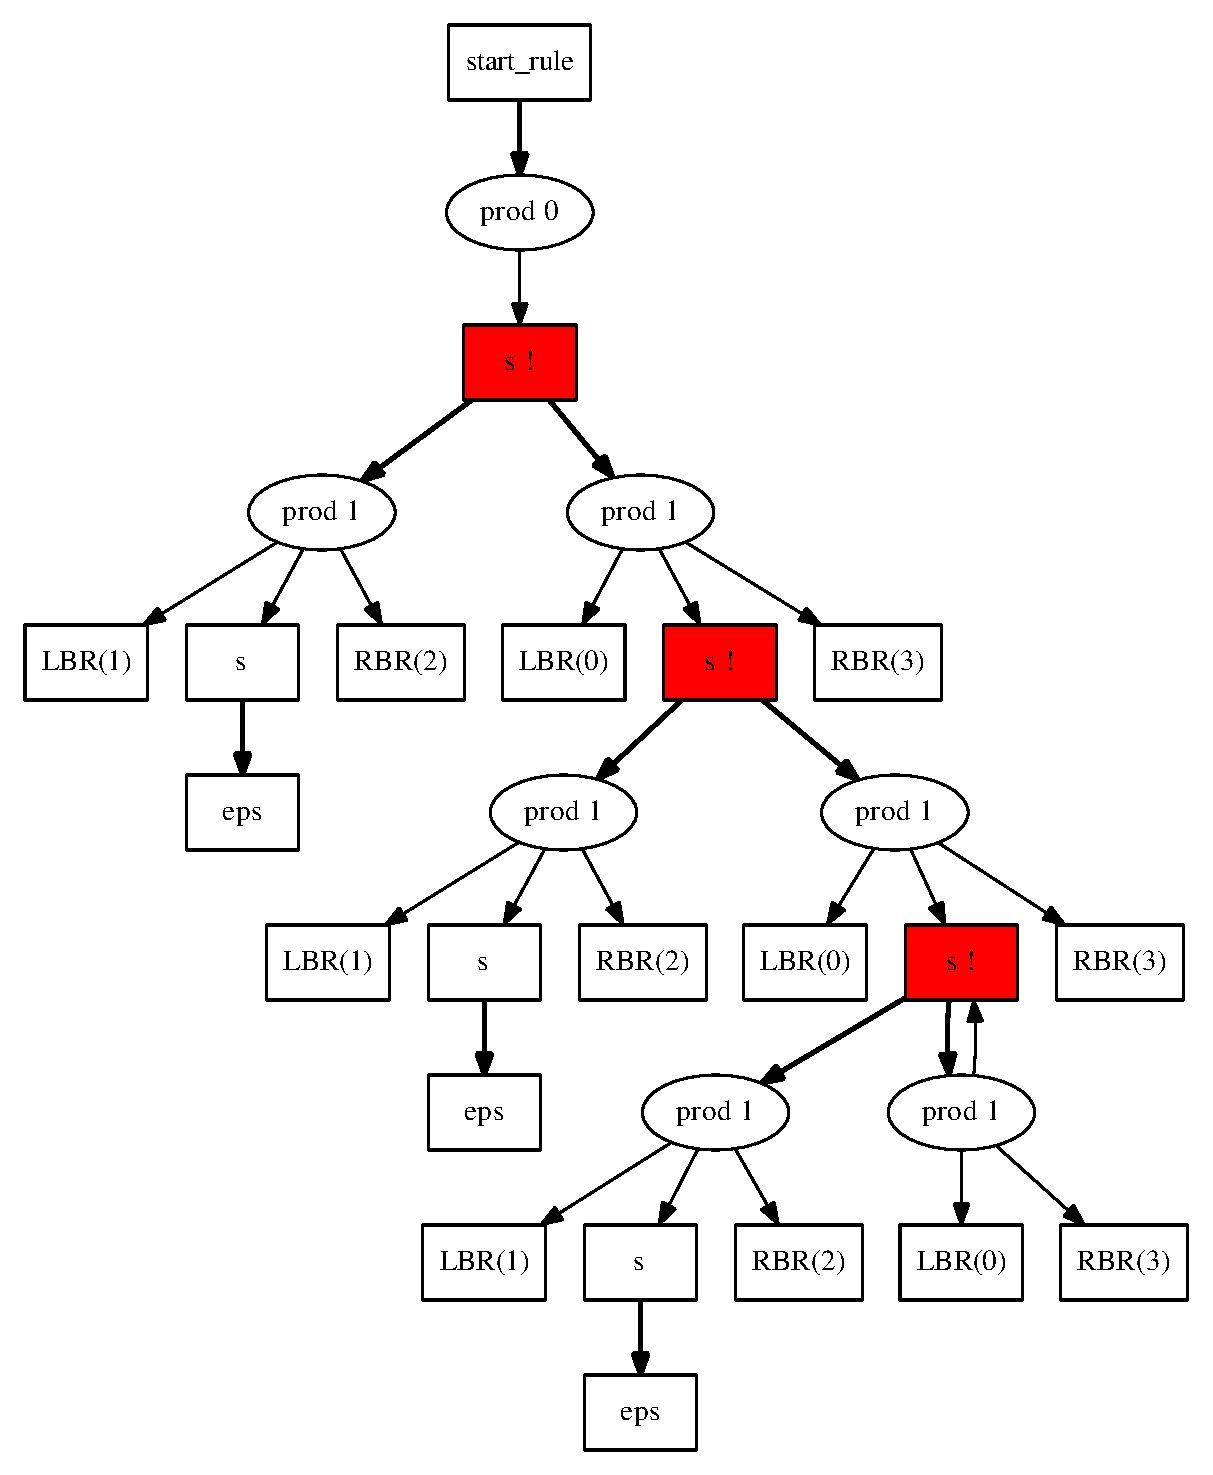
\includegraphics[scale=0.3]{dot/out3.eps}
    }
    \caption{Regular approximation and SPPF}
    \label{fig:SPPFforReg}
 \end{figure}

%\begin{figure}
%    \begin{center}
%        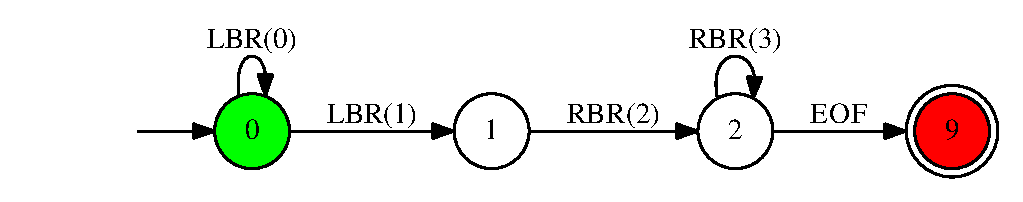
\includegraphics[scale=0.5]{dot/in3.eps}
%    \end{center}
%    \caption{$A_1$ -- input for our algorithm: regular approximation for string-embedded code after tokenization} 
%    \label{faApprox}
%\end{figure}

As it can be seen, some of the words from regular approximation do not belong to the reference language (for example, 
\verb|LBR LBR RBR|). The algorithm ignores such strings and constructs SPPF, which contains derivation trees 
for all recognized strings w.r.t. reference grammar.

%\begin{figure}
%    \begin{center}
%        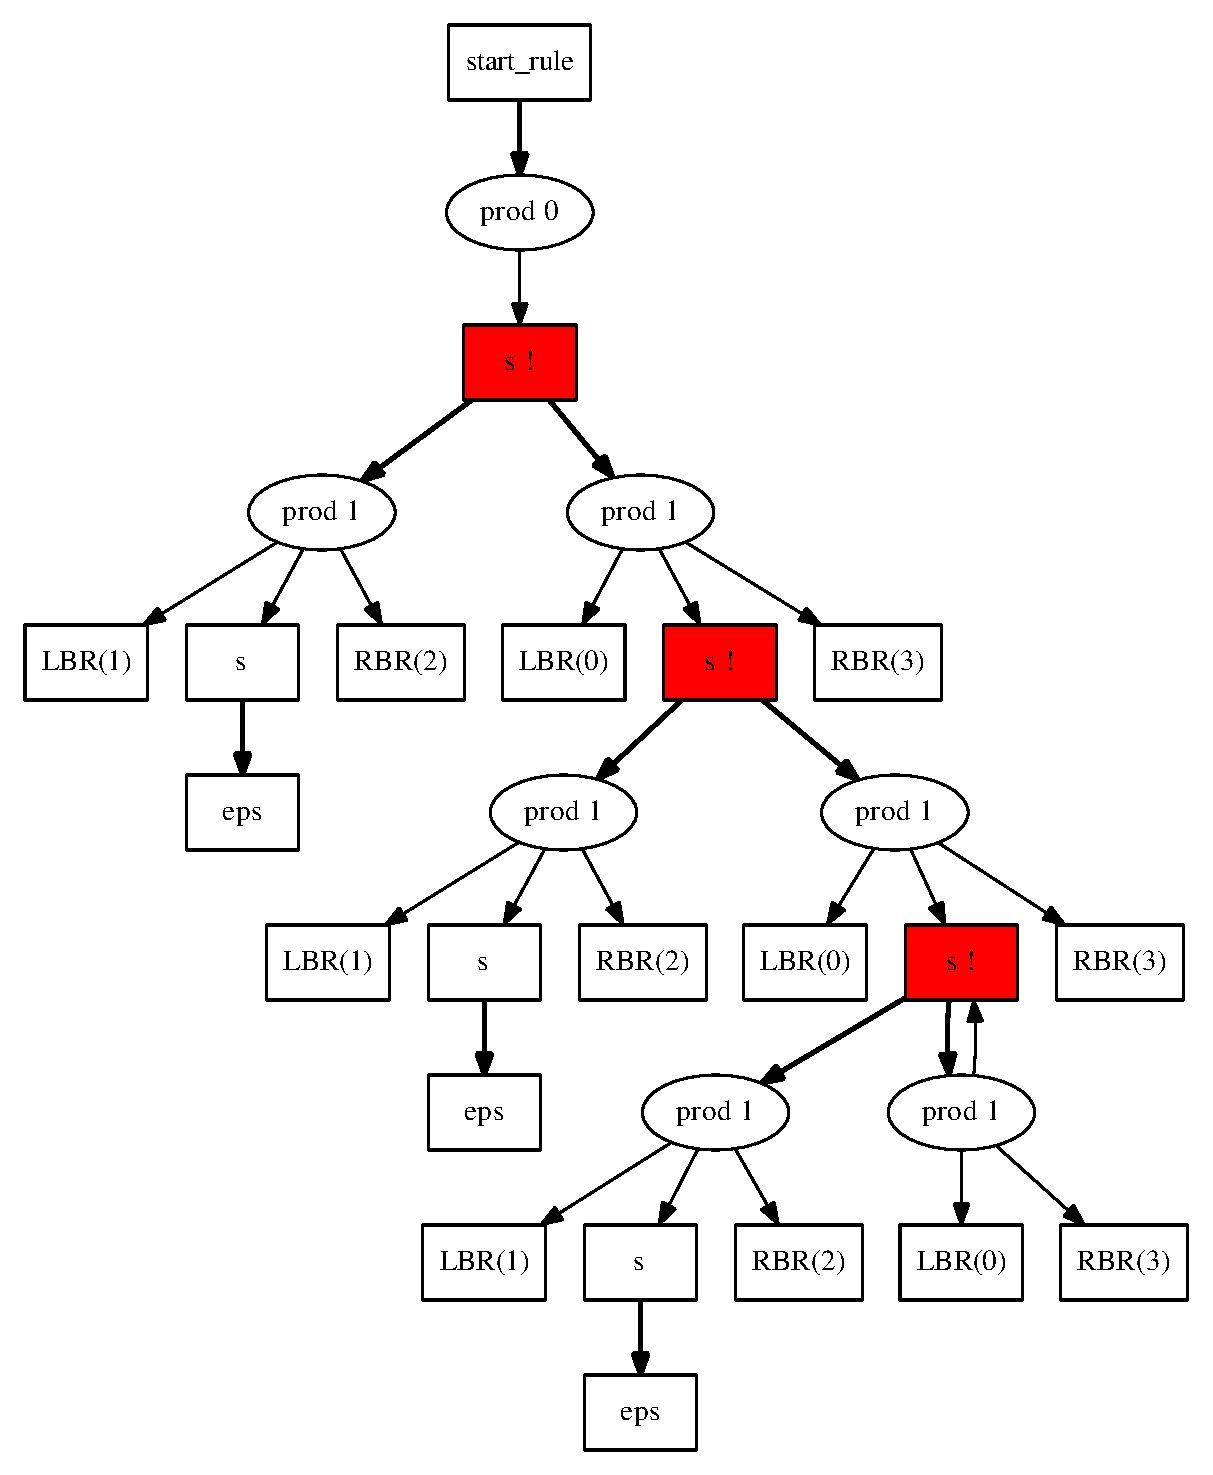
\includegraphics[scale=0.3]{dot/out3.eps}
%    \end{center}
%    \caption{SPPF for input FA presented in figure~\ref{faApprox}}
%    \label{resultSPPF}
%\end{figure}
\pagebreak
\section{\appendixname: RNGLR pseudocode}\label{RNGLRCode}

\begin{algorithm}[]
\begin{algorithmic}[1]
\caption{RNGLR algorithm}
\label{rnglr}
\Function{parse}{$grammar, input$}
  \State{$\mathcal{R} \gets \emptyset$} \Comment{Queue of tuples of GSS vertex, nonterminal, and reduction length}
  \State{$\mathcal{Q} \gets \emptyset$} \Comment{Collection of pairs of GSS vertex and parser state}
  \If{$input = \epsilon$}
    \If{$grammar$ accepts empty input} {report success}
    \Else { report failure}
    \EndIf
  \Else
    \State{\Call{addVertex}{$0, 0, startState$}}
    \ForAll{$i$ in $0..input.Length-1$}
      \State{\Call{reduce}{$i$}}
      \State{\Call{push}{$i$}}
    \EndFor
    \If{$i=input.Length-1$ and there is a vertex in the last level of GSS which state is accepting}
      \State{report success}
    \Else { report failure}
    \EndIf
  \EndIf
\EndFunction
\Function{reduce}{$i$}
  \While{$\mathcal{R}$ is not empty}
    \State{$(v, N, l) \gets \mathcal{R}.Dequeue()$}
    \State{find the set $\mathcal{X}$ of vertices reachable from $v$ along the path of length $(l-1)$}
    \State{or length $0$ if $l=0$}
    \ForAll{$v_{h} = (level_{h}, state_{h})$ in $\mathcal{X}$}
      \State{$state_{t} \gets$ calculate new state by $state_{h}$ and nonterminal $N$}
      \State{\Call{addEdge}{$i, v_{h}, v.level, state_{tail}, (l=0)$}}
    \EndFor
  \EndWhile
\EndFunction
\Function{push}{$i$}
  \State{$\mathcal{Q^{'}} \gets$ copy $\mathcal{Q}$}
  \While{$\mathcal{Q^{'}}$ is not empty}
    \State{$(v, state) \gets \mathcal{Q}.Dequeue()$}
    \State{\Call{addEdge}{$i, v, v.level + 1, state, false$}}
  \EndWhile
\EndFunction
\end{algorithmic}
\end{algorithm}

\begin{algorithm}[]
\begin{algorithmic}[1]
\caption{GSS construction}
\label{RNGLRMain}
\Function{addVertex}{$i, level, state$}
  \If{GSS does not contain vertex $v = (level, state)$}
    \State{add new vertex $v = (level, state)$ to GSS}
    \State{calculate the set of shifts by $v$ and the $input[i+1]$ and add them to $\mathcal{Q}$}
    \State{calculate the set of zero-reductions by $v$ and the $input[i+1]$ and}
    \State{add them to $\mathcal{R}$}
  \EndIf
  \State{\Return{$v$}}
\EndFunction
\Function{addEdge}{$i, v_{h}, level_{t}, state_{t}, isZeroReduction$}
  \State{$v_{t} \gets$ \Call{addVertex}{$i, level_{t}, state_{t}$}}
  \If{GSS does not contain edge from $v_{t}$ to $v_{h}$}
    \State{add new edge from $v_{t}$ to $v_{h}$ to GSS}
    \If{not $isZeroReduction$}
      \State{calculate the set of reductions by $v$ and the $input[i+1]$ and}
      \State{add them to $\mathcal{R}$}
    \EndIf
  \EndIf
\EndFunction
\end{algorithmic}
\end{algorithm}



\end{document}
